\documentclass{beamer}
\usepackage{listings}
\usepackage[font=small]{caption}
\usepackage[outdir=./images/]{epstopdf}
\definecolor{codegreen}{rgb}{0,0.6,0}
\definecolor{codegray}{rgb}{0.5,0.5,0.5}
\definecolor{codepurple}{rgb}{0.58,0,0.82}
\definecolor{backcolour}{rgb}{0.95,0.95,0.92}


\lstdefinestyle{mystyle}{
	backgroundcolor=\color{backcolour},
	commentstyle=\color{codegreen},
	keywordstyle=\color{magenta},
	numberstyle=\tiny\color{codegray},
	stringstyle=\color{codepurple},
	basicstyle=\ttfamily\footnotesize,
	breakatwhitespace=false,
	breaklines=true,
	captionpos=b,
	keepspaces=true,
	numbers=left,
	numbersep=5pt,
	showspaces=false,
	showstringspaces=false,
	showtabs=false,
	tabsize=2
}
\lstset{style=mystyle}


\usetheme{Frankfurt}
\beamertemplatenavigationsymbolsempty

\title{jaxFlowSim}

\author{Diego Renner}

\begin{document}

\section{Introduction}
\maketitle

\begin{frame}
	\frametitle{Introduction}
	\begin{block}{What is jaxFlowSim?}
		\begin{itemize}
			\item 1D-haemodynamics solver
			\item written in JAX
			\item differentiable
		\end{itemize}
	\end{block}
	\vspace{5mm}
\end{frame}

\begin{frame}
	\frametitle{Motivation}
	\begin{block}{Use and Novelty}
		\begin{itemize}
			\item towards personalised medicine
			\item parameter inference
			\item sensitivity analysis
		\end{itemize}
	\end{block}
	\vspace{5mm}
\end{frame}

\section{Model}

\begin{frame}
	\frametitle{1D-Navier Stokes Equations}
	pde with boundary/initial conditions
\end{frame}
\begin{frame}
	\frametitle{Inlets}
	example computing inlets from data
\end{frame}
\begin{frame}
	\frametitle{Junctions}
	exmaple of linear system for junction
\end{frame}
\begin{frame}
	\frametitle{Outlets}
	description of Windkessel model
\end{frame}

\section{Implementation}

\begin{frame} [fragile]
	\frametitle{Code Structure}
	\begin{lstlisting}[basicstyle=\fontsize{7}{7}\selectfont\ttfamily, language=Python, caption={$dt \hat{=}$timestep(CFL), setBoundaryValues$\hat{=}$inlet(from data), outlet(Windkessel),junctions(conservation laws), muscl$\hat{=}$Monotonic Upstream-centered Scheme for Conservation Laws(Finite Volume)}, label=lst:pc, escapechar=|] 
		def runSimulation(config_filename, J) 
			config = loadConfig(config_filename) |\label{ln:init_start}|
			simulation_data = buildArterialNetwork(config) |\label{ln:init_end}|

			P_t = [0] |\label{ln:pt}|

			converged = False |\label{ln:whout1}|
			while not converged: |\label{ln:whout2}|
				t = 0 |\label{ln:t0}|
				i = 0 |\label{ln:i0}|
				P_t_temp = P_t |\label{ln:cp}|
				while t < T:
					dt = computeDt(simulation_data) |\label{ln:cfl}|
					simulation_data = setBoundaryValues(simulation_data, dt) |\label{ln:bv    }|
					simulation_data = muscl(simulation_data, dt) |\label{ln:muscl}|
					P_t[i,:] = savePressure(simulation_data) |\label{ln:svp}|
					t = t + dt |\label{ln:updt}|
				i = i + 1 |\label{ln:updi}|
				if i >= J:
					break
				converged = checkConv(P_t, P_t_temp) |\label{ln:conv}|
\end{lstlisting}
\end{frame}
\begin{frame}
	\frametitle{Padding}
	without padding
	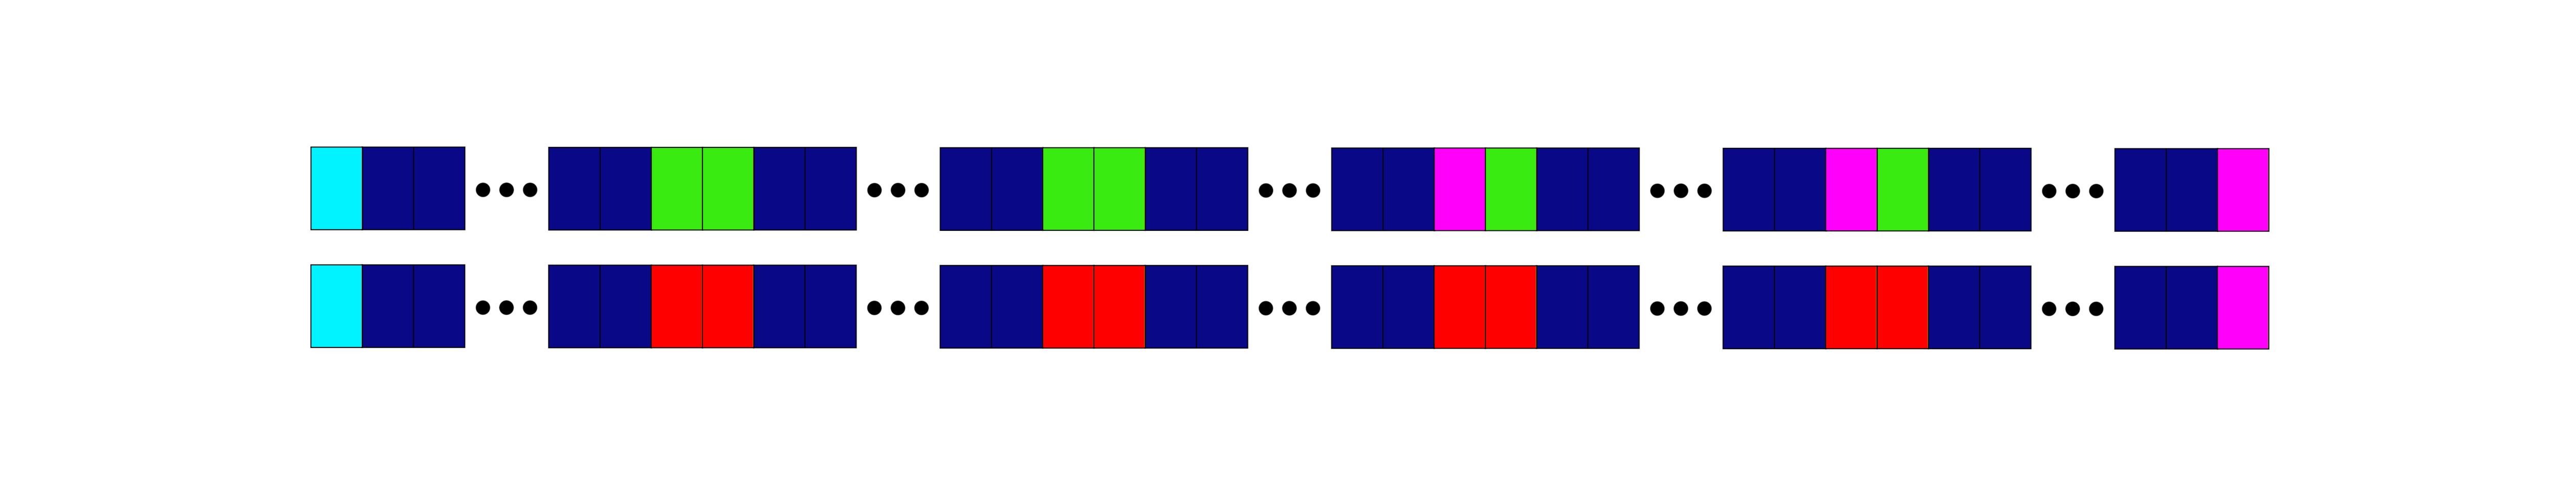
\includegraphics[width=\textwidth]{images/padding1.eps}
	with padding
	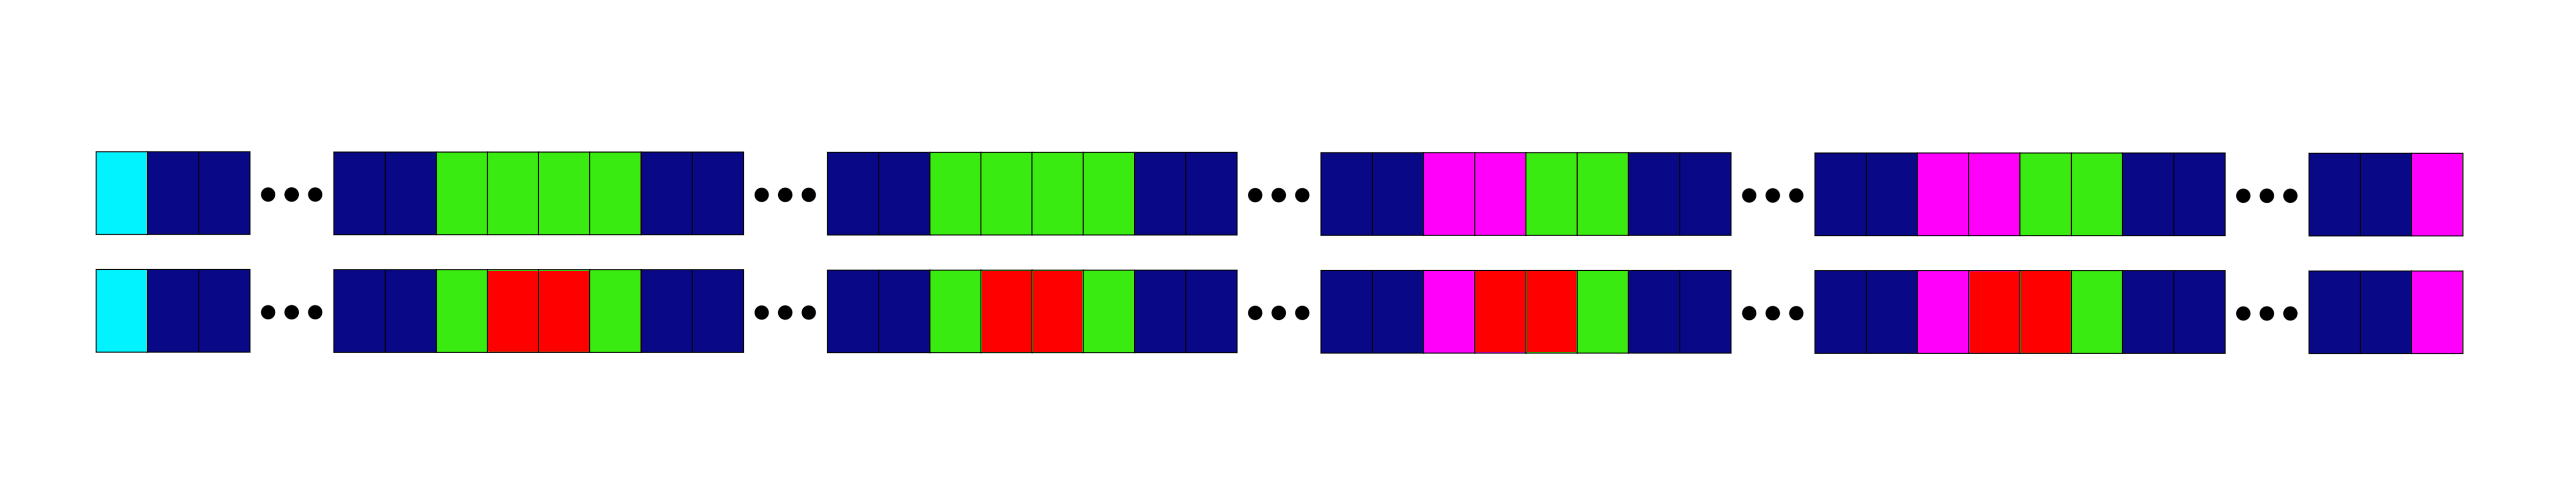
\includegraphics[width=\textwidth]{images/padding2.eps}
	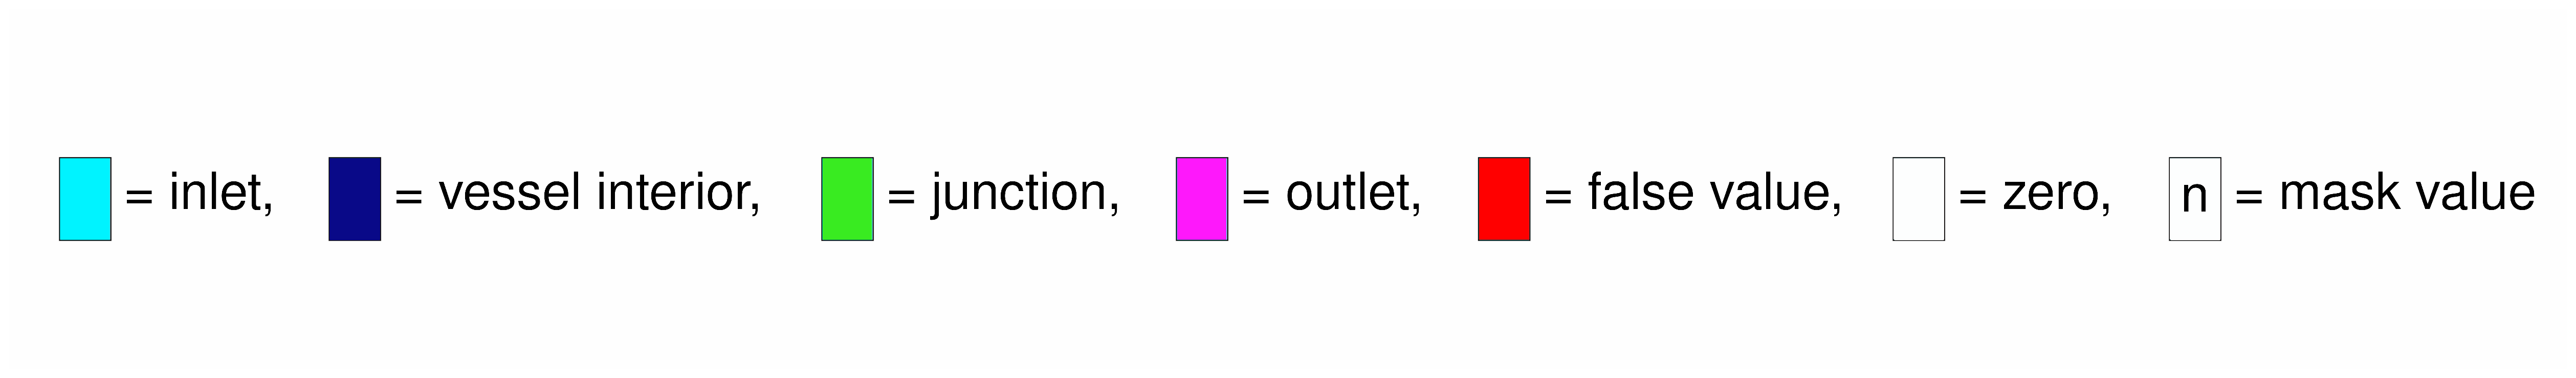
\includegraphics[width=\textwidth]{images/legend.eps}
\end{frame}
\begin{frame}
	\frametitle{Masking}
	\includegraphics[width=\textwidth]{images/masking.eps}
	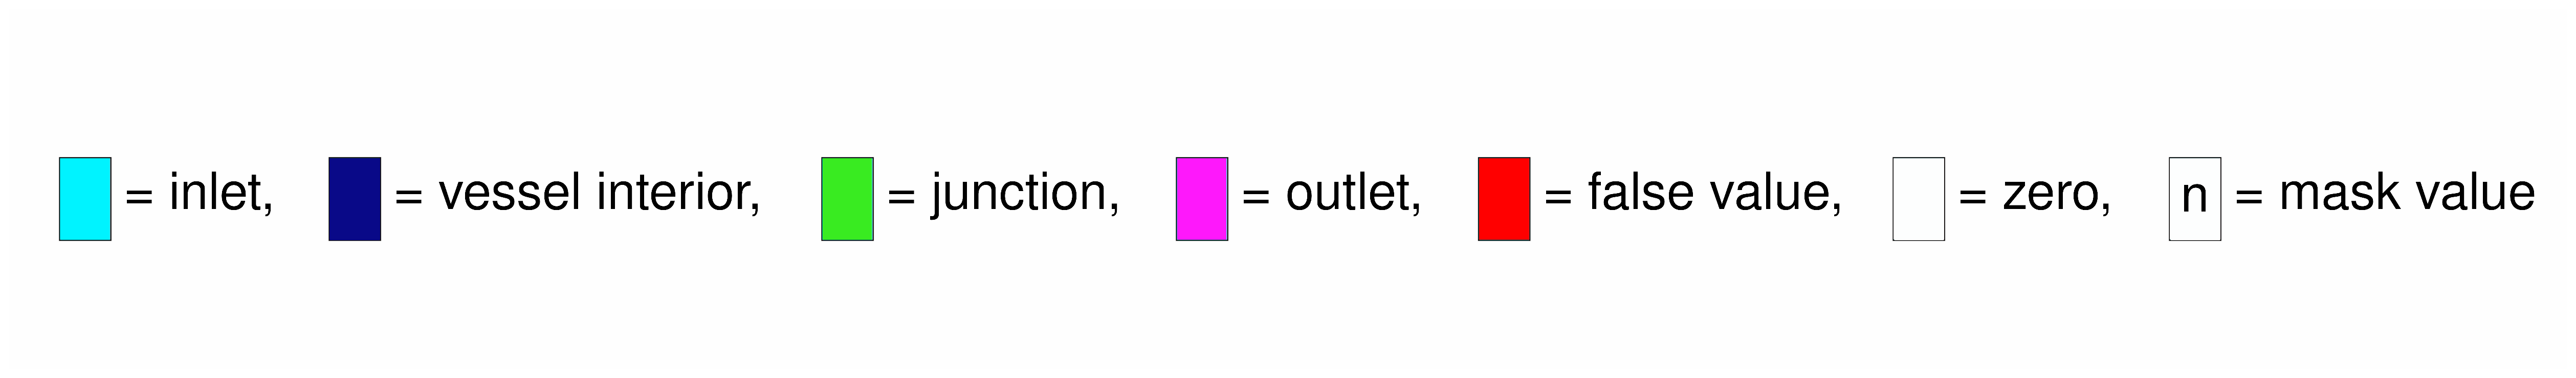
\includegraphics[width=\textwidth]{images/legend.eps}
\end{frame}

\section{Results}
\begin{frame}
	\frametitle{Model: Aorta (0007\_H\_AO\_H)}
	\begin{figure} [H]
		\centering
		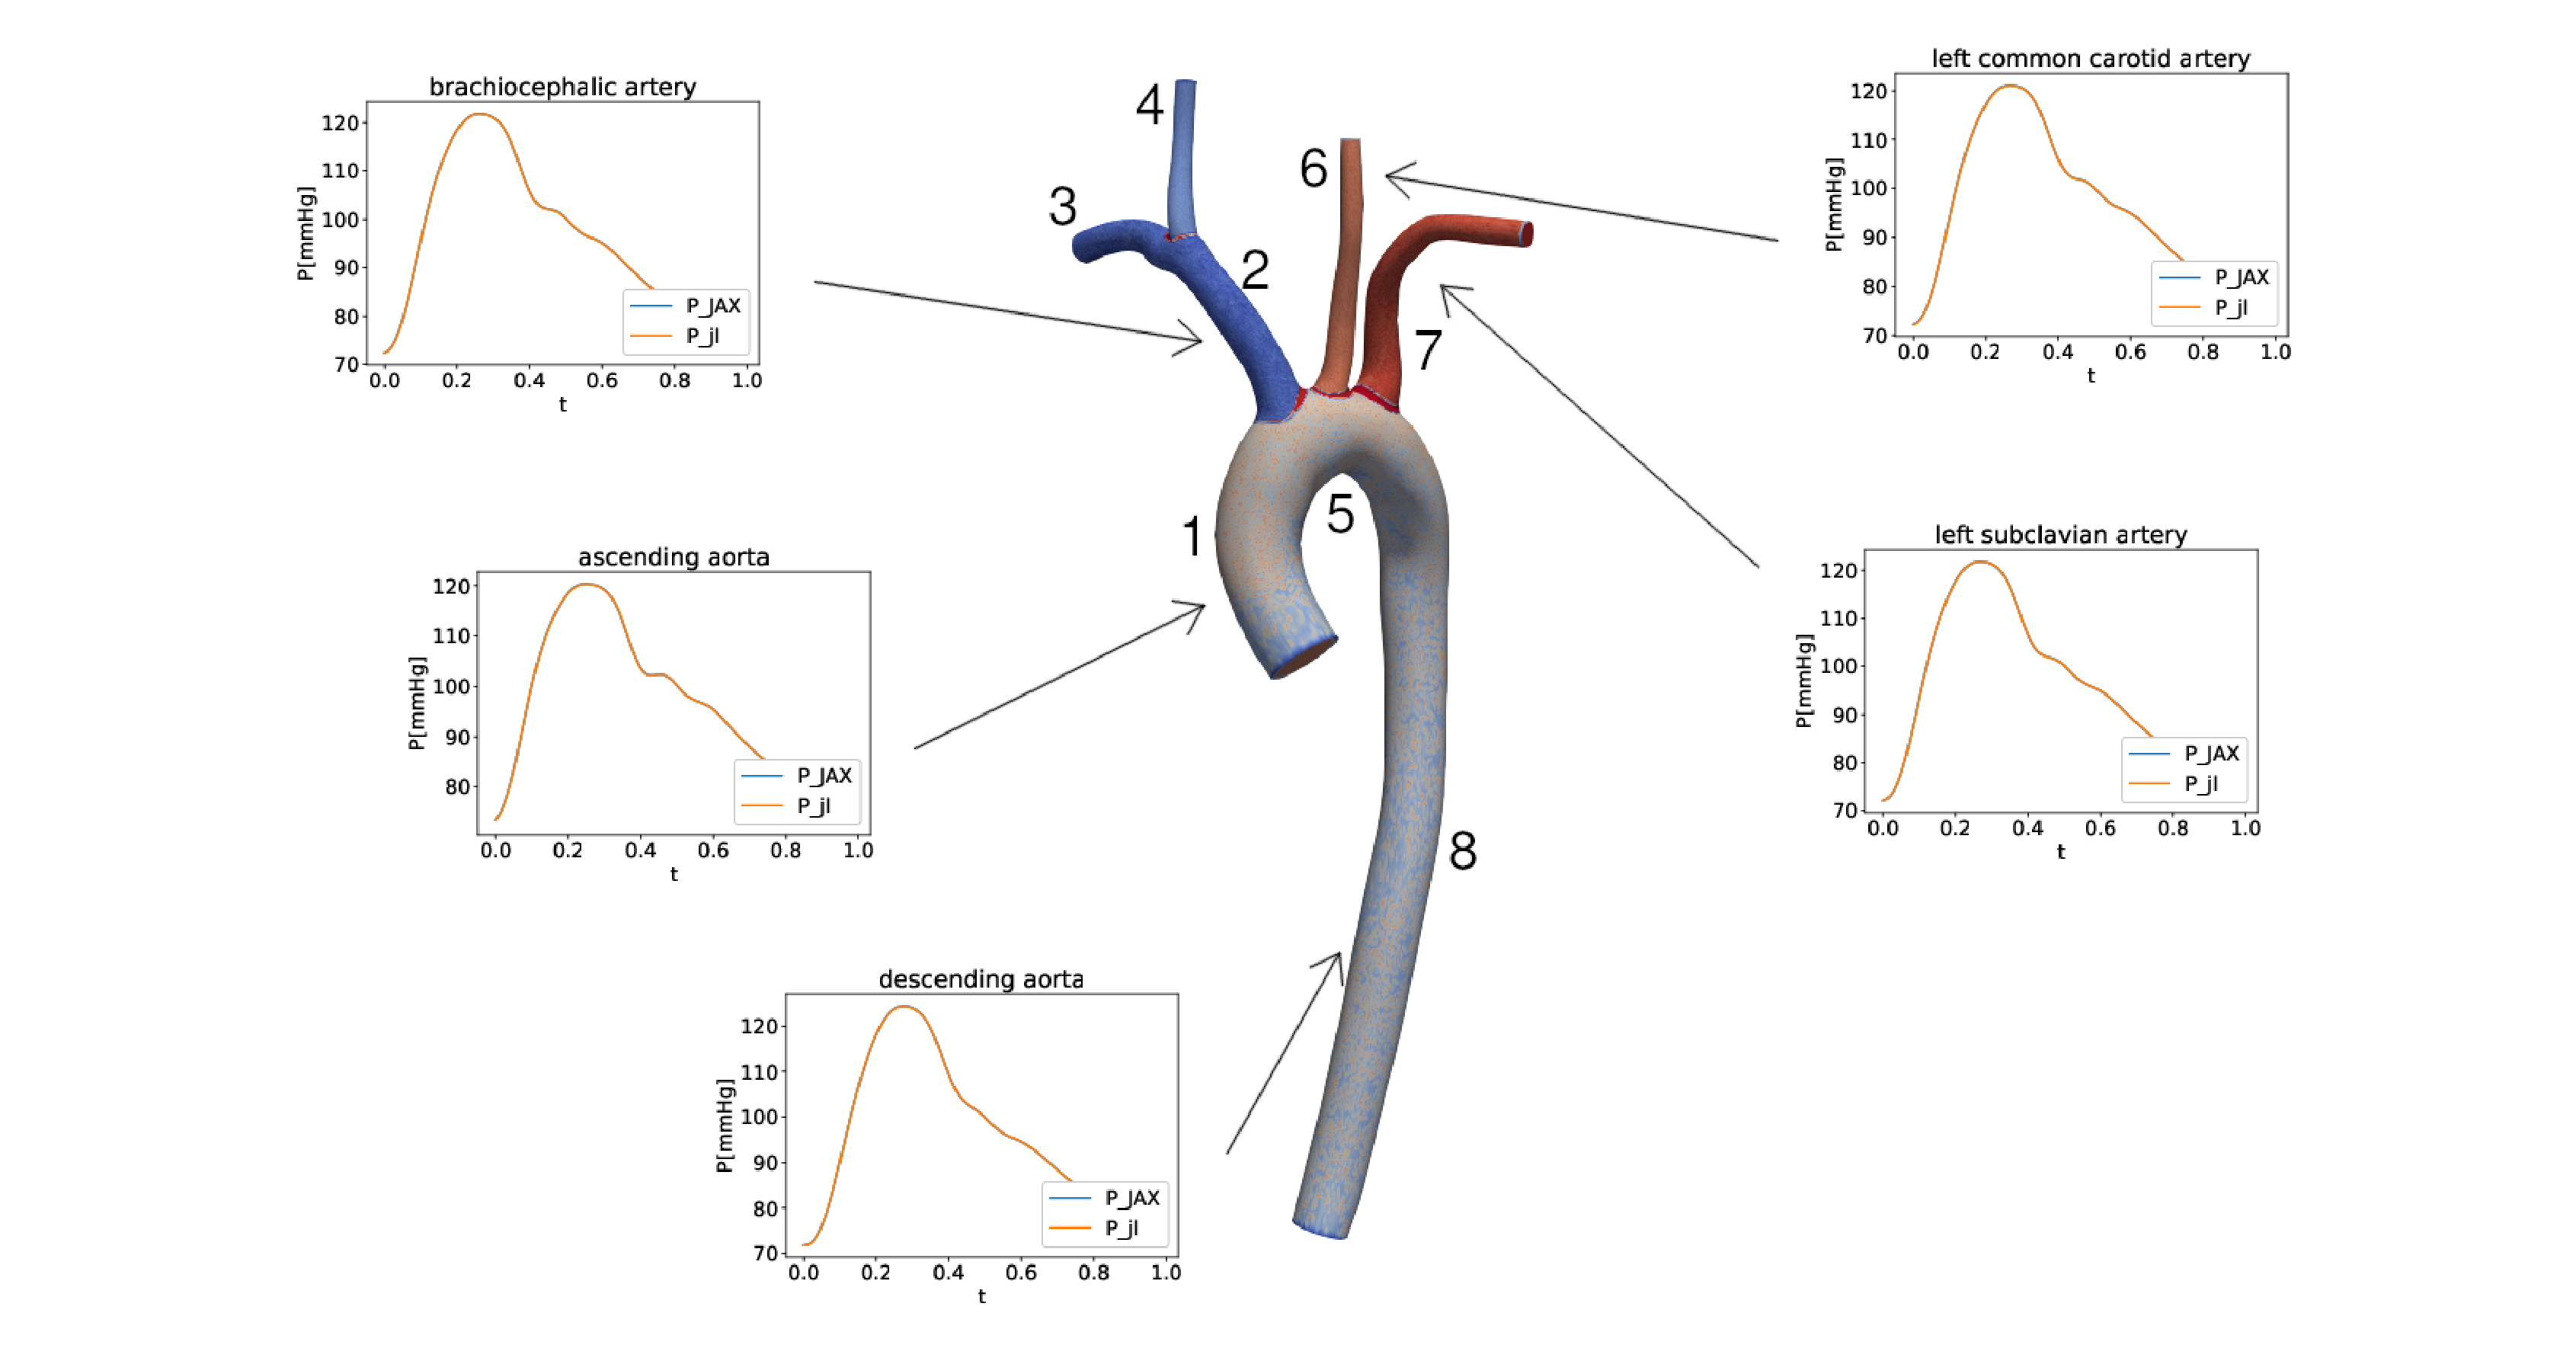
\includegraphics[width=\columnwidth]{images/0007.eps}
		\label{fig:aorta}
	\end{figure}
\end{frame}
\begin{frame}
	\frametitle{Model: Abdominal Arteries (0029\_H\_ABAO\_H)}
		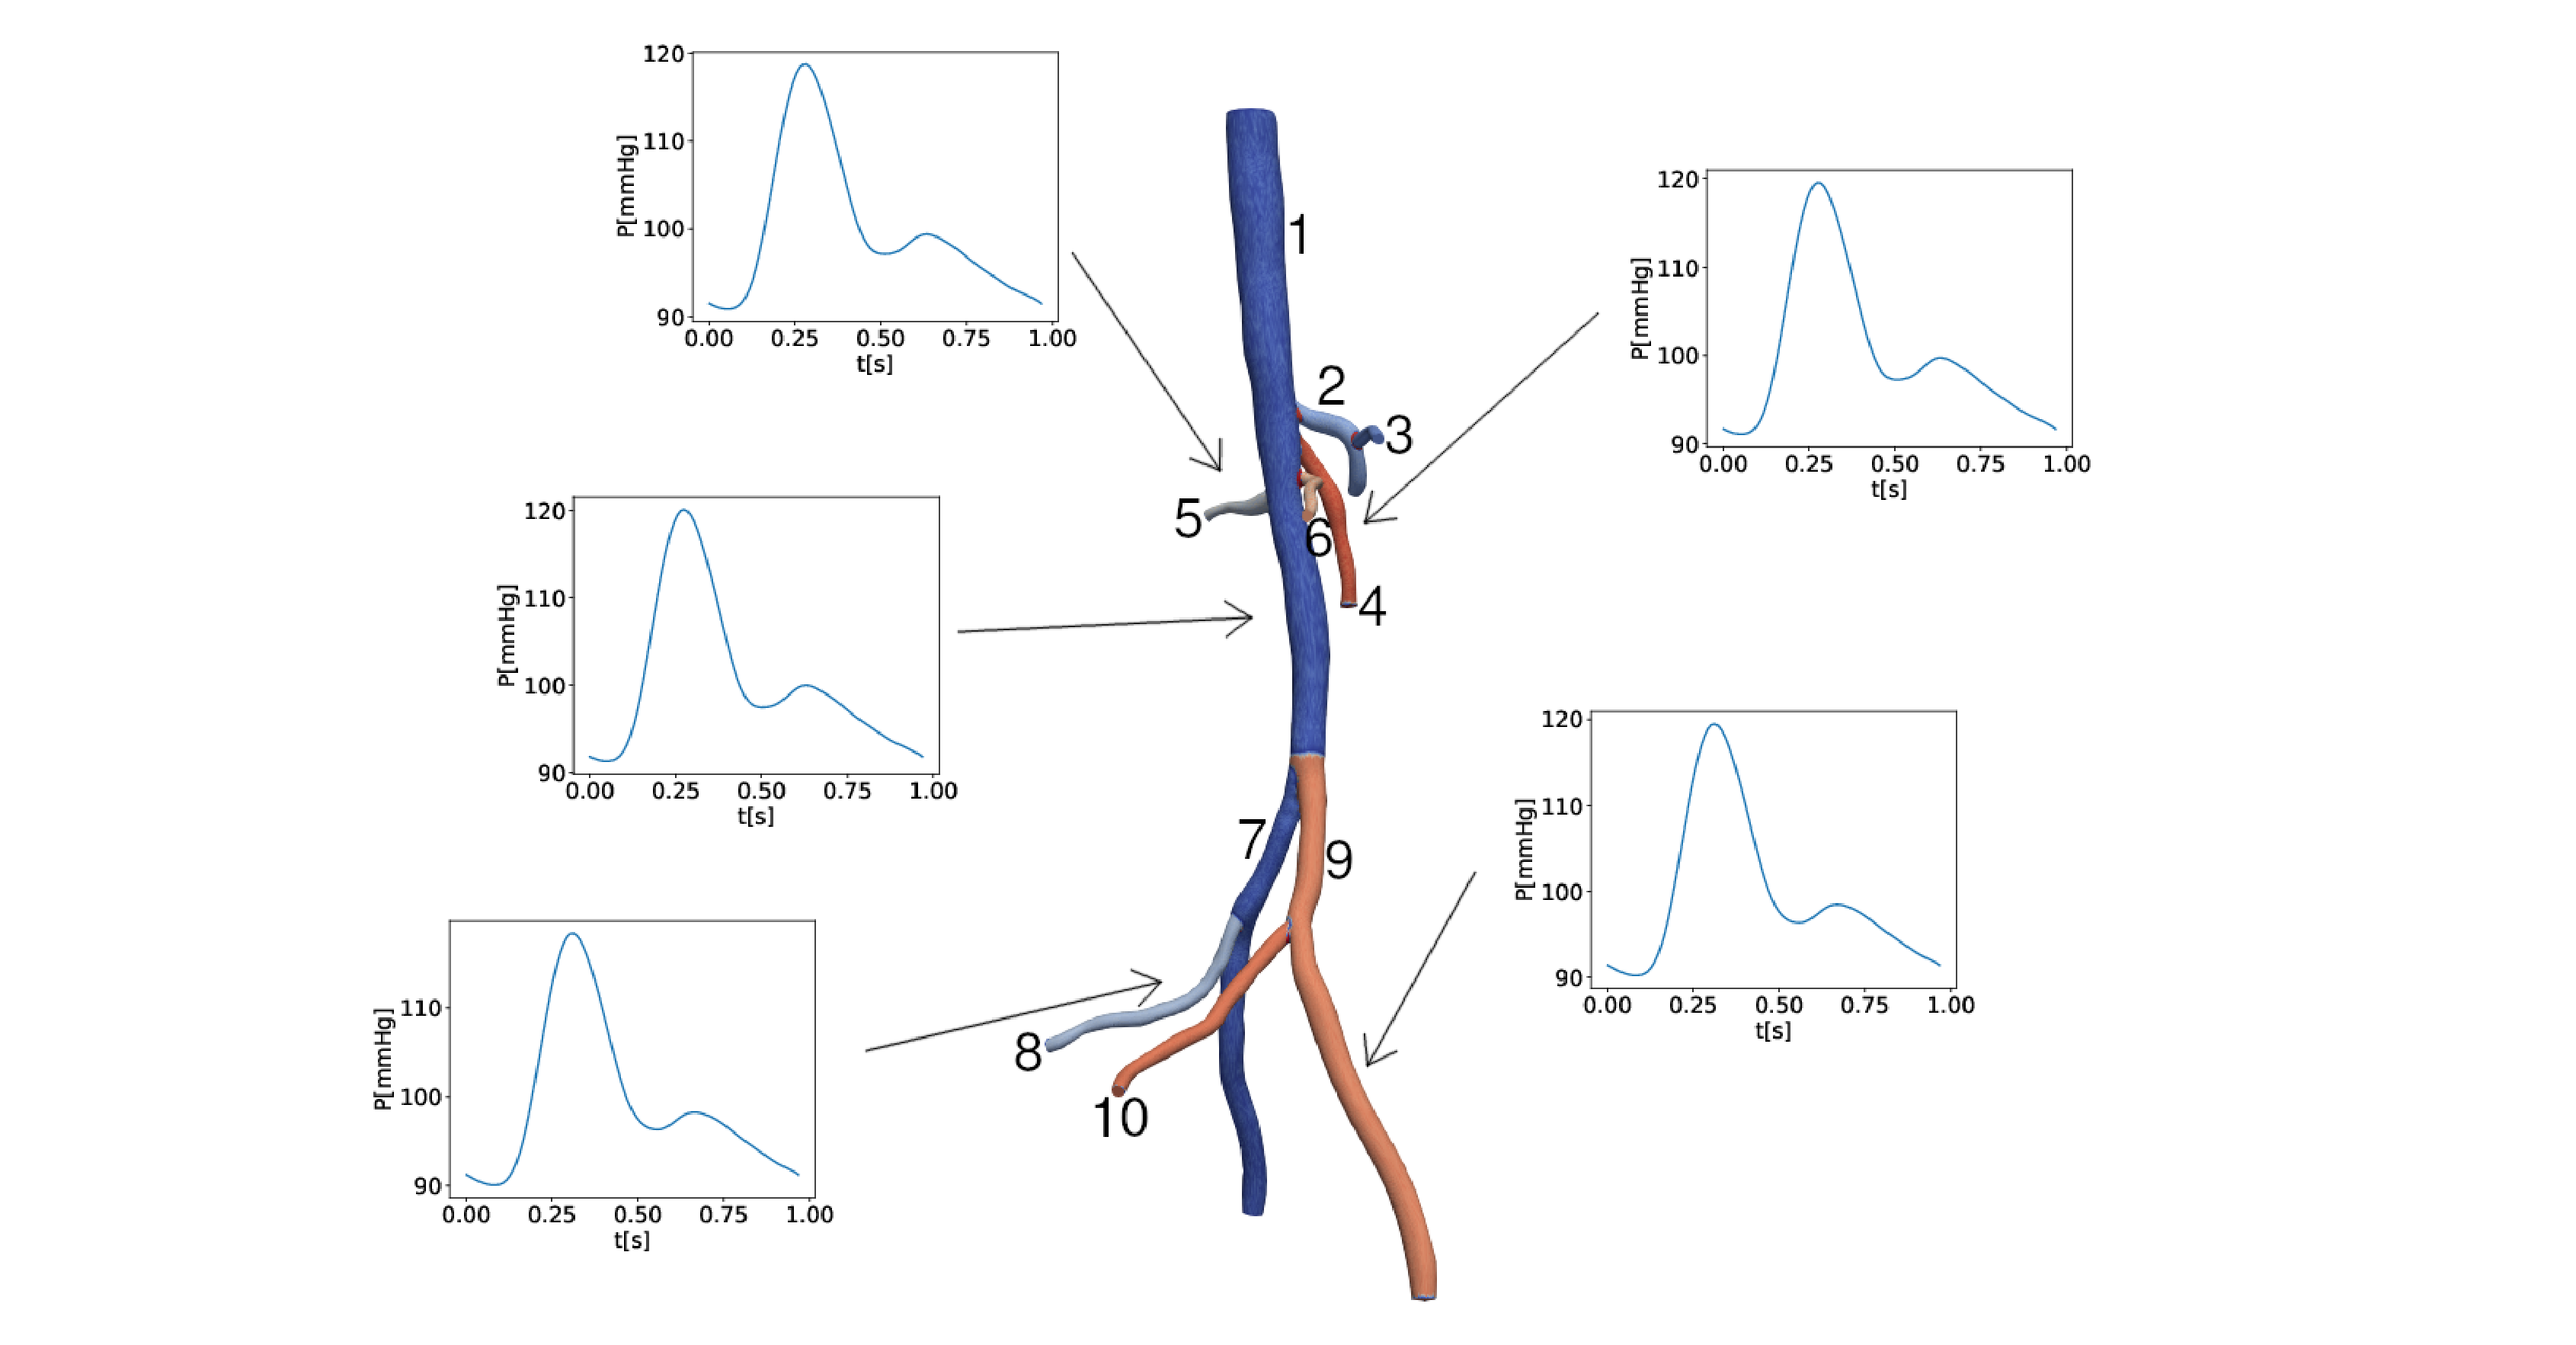
\includegraphics[width=\columnwidth]{images/0029.eps}
\end{frame}
\begin{frame}
	\frametitle{Model: Cerebellar Arteries (0053\_H\_CERE\_H)}
	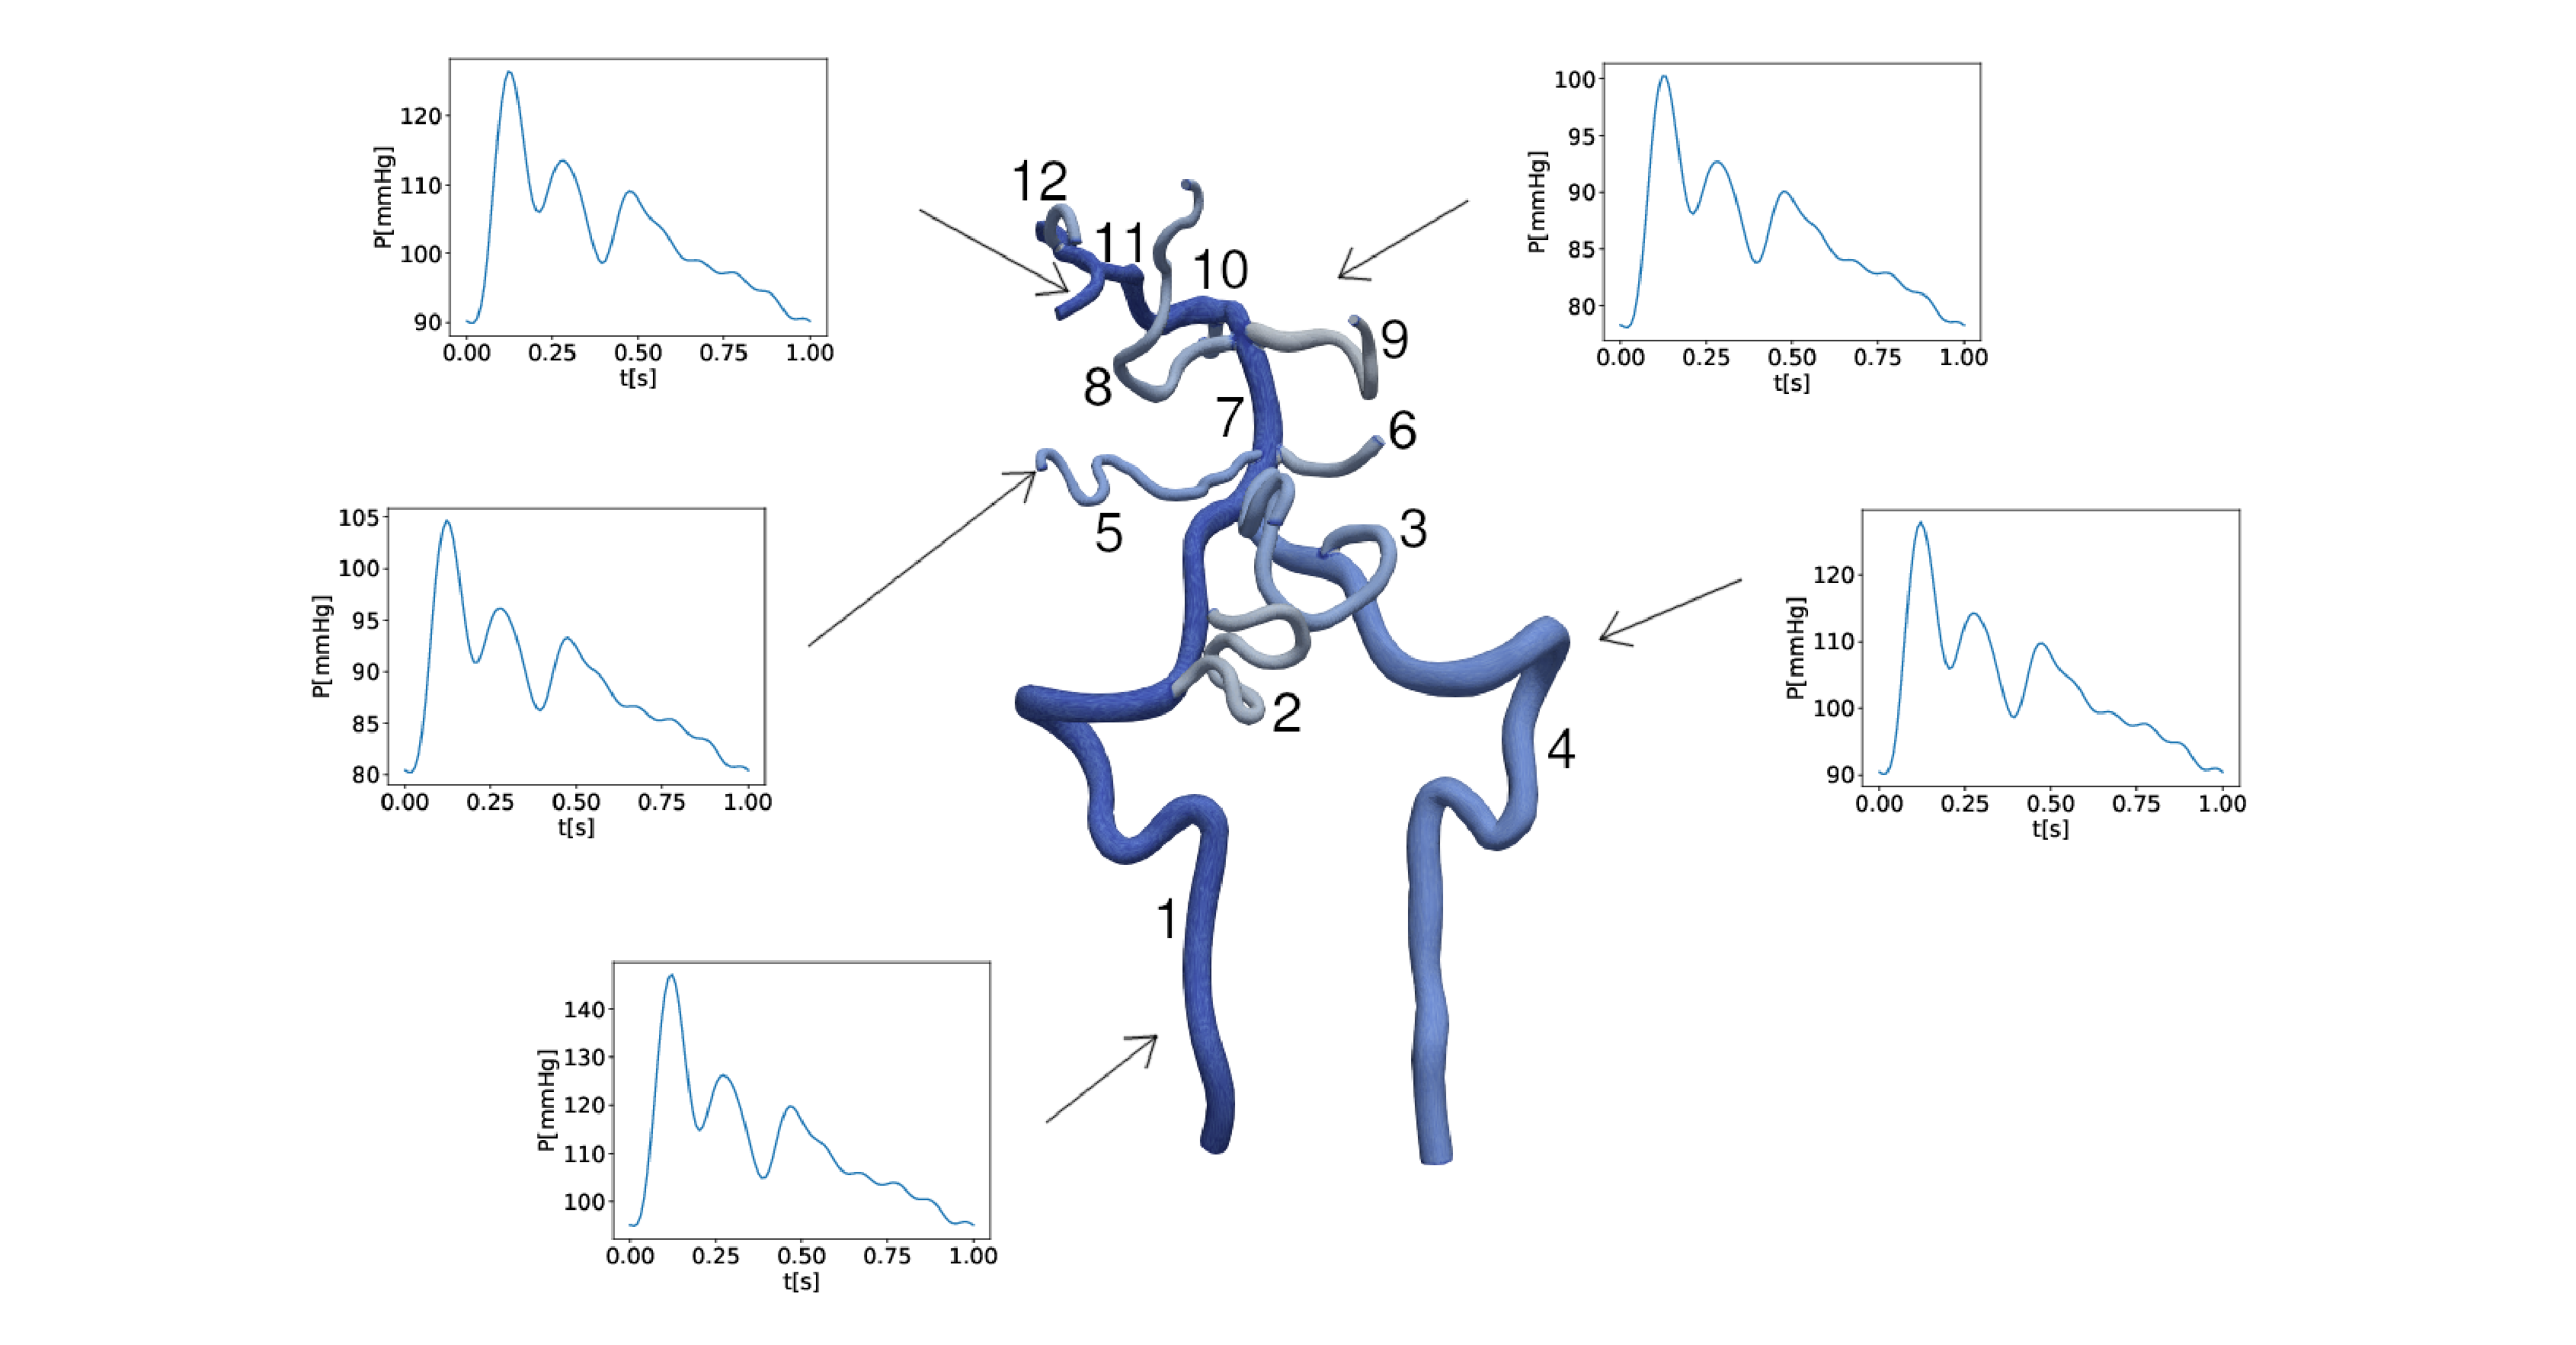
\includegraphics[width=\columnwidth]{images/0053.eps}
\end{frame}
\begin{frame}
	\frametitle{Model: ADAN56}
	\includegraphics[width=\textwidth]{images/adan56_annotated.png}
\end{frame}
\begin{frame}
	\frametitle{Validation}
	\begin{figure} [H]
		\centering
		\includegraphics[width=0.46\columnwidth]{images/0007_H_AO_H_right_subclavian_artery_P.eps}
		\includegraphics[width=0.46\columnwidth]{images/0029_H_ABAO_H_celiac_branch_P.eps
		}
		\includegraphics[width=0.46\columnwidth]{images/0053_H_CERE_H_basilar_artery_IV_P.eps}
		\includegraphics[width=0.46\columnwidth]{images/adan56_common_hepatic_P.eps}
		\label{fig:val}
	\end{figure}
\end{frame}
\begin{frame}
	\frametitle{Comparison}
	\begin{figure} [H]
		\centering
		\includegraphics[width=0.94\columnwidth]{images/comparison.eps}
		\label{fig:comparison}
	\end{figure}

\end{frame}
\begin{frame}
	\frametitle{Inference}
	\begin{block}{Demo}
		inferring an outlet resistance parameter from precomputed data
	\end{block}
\end{frame}

\section{Future Work}
\begin{frame}
	\frametitle{Future Work}
	\begin{block}{Main Points of Interest}
		\begin{itemize}
			\item improving performance (GPU optimization)
			\item fine tuning parameter inference
			\item sensitivity analysis
		\end{itemize}
	\end{block}
	\vspace{5mm}
\end{frame}

\begin{frame}
	\frametitle{Questions?}
	Thank you for your attention!
\end{frame}

\end{document}
